%%%%%%%%%%%%%%%%%%%%%%%%%%%%%%%%%%%%%%%%%
% Beamer Presentation
% LaTeX Template
% Version 1.0 (10/11/12)
%
% This template has been downloaded from:
% http://www.LaTeXTemplates.com
%
% License:
% CC BY-NC-SA 3.0 (http://creativecommons.org/licenses/by-nc-sa/3.0/)
%
%%%%%%%%%%%%%%%%%%%%%%%%%%%%%%%%%%%%%%%%%

%----------------------------------------------------------------------------------------
%	PACKAGES AND THEMES
%----------------------------------------------------------------------------------------

\documentclass{beamer}

\mode<presentation> {

% The Beamer class comes with a number of default slide themes
% which change the colors and layouts of slides. Below this is a list
% of all the themes, uncomment each in turn to see what they look like.

%\usetheme{default}
%\usetheme{AnnArbor}
%\usetheme{Antibes}
%\usetheme{Bergen}
%\usetheme{Berkeley}
%\usetheme{Berlin}
%\usetheme{Boadilla}
%\usetheme{CambridgeUS}
%\usetheme{Copenhagen}
%\usetheme{Darmstadt}
%\usetheme{Dresden}
%\usetheme{Frankfurt}
%\usetheme{Goettingen}
%\usetheme{Hannover}
%\usetheme{Ilmenau}
%\usetheme{JuanLesPins}
%\usetheme{Luebeck}
\usetheme{Madrid}
%\usetheme{Malmoe}
%\usetheme{Marburg}
%\usetheme{Montpellier}
%\usetheme{PaloAlto}
%\usetheme{Pittsburgh}
%\usetheme{Rochester}
%\usetheme{Singapore}
%\usetheme{Szeged}
%\usetheme{Warsaw}

% As well as themes, the Beamer class has a number of color themes
% for any slide theme. Uncomment each of these in turn to see how it
% changes the colors of your current slide theme.

%\usecolortheme{albatross}
%\usecolortheme{beaver}
%\usecolortheme{beetle}
%\usecolortheme{crane}
%\usecolortheme{dolphin}
%\usecolortheme{dove}
%\usecolortheme{fly}
%\usecolortheme{lily}
%\usecolortheme{orchid}
%\usecolortheme{rose}
%\usecolortheme{seagull}
%\usecolortheme{seahorse}
\usecolortheme{whale}
%\usecolortheme{wolverine}

\setbeamertemplate{footline} % To remove the footer line in all slides uncomment this line
%\setbeamertemplate{footline}[page number] % To replace the footer line in all slides with a simple slide count uncomment this line

\setbeamertemplate{navigation symbols}{} % To remove the navigation symbols from the bottom of all slides uncomment this line

}

\usepackage{graphicx} % Allows including images
\usepackage{booktabs} % Allows the use of \toprule, \midrule and \bottomrule in tables
\usepackage{sansmathaccent}
\usepackage{amsmath}
\pdfmapfile{+sansmathaccent.map}

\usepackage{tikz}
\usetikzlibrary{trees, arrows, shapes, positioning}
%----------------------------------------------------------------------------------------
%	TITLE PAGE
%----------------------------------------------------------------------------------------

\title[]{Hard Problems} % The short title appears at the bottom of every slide, the full title is only on the title page

%\author{John Smith} % Your name
\institute[BYU] % Your institution as it will appear on the bottom of every slide, may be shorthand to save space
{
Brigham Young University \\ % Your institution for the title page
\medskip
%\textit{john@smith.com} % Your email address
}
\date{\today} % Date, can be changed to a custom date

\begin{document}

\begin{frame}
\titlepage % Print the title page as the first slide
\end{frame}

%\begin{frame}
%\frametitle{Overview} % Table of contents slide, comment this block out to remove it
%\tableofcontents % Throughout your presentation, if you choose to use \section{} and %\subsection{} commands, these will automatically be printed on this slide as an overview of your presentation
%\end{frame}

%----------------------------------------------------------------------------------------
%	PRESENTATION SLIDES
%----------------------------------------------------------------------------------------

%------------------------------------------------
%\section{First Section} % Sections can be created in order to organize your presentation into %discrete blocks, all sections and subsections are automatically printed in the table of contents %as an overview of the talk
%------------------------------------------------

%\subsection{Subsection Example} % A subsection can be created just before a set of slides with %a common theme to further break down your presentation into chunks

%\begin{frame}
%\frametitle{AVL trees}
%Sed iaculis dapibus gravida. Morbi sed tortor erat, nec interdum arcu. Sed id lorem lectus. %Quisque viverra augue id sem ornare non aliquam nibh tristique. Aenean in ligula nisl. Nulla sed %tellus ipsum. Donec vestibulum ligula non lorem vulputate fermentum accumsan neque mollis.%\\~\\

%Sed diam enim, sagittis nec condimentum sit amet, ullamcorper sit amet libero. Aliquam vel dui %orci, a porta odio. Nullam id suscipit ipsum. Aenean lobortis commodo sem, ut commodo leo %gravida vitae. Pellentesque vehicula ante iaculis arcu pretium rutrum eget sit amet purus. %Integer ornare nulla quis neque ultrices lobortis. Vestibulum ultrices tincidunt libero, quis %commodo erat ullamcorper id.
%\end{frame}
%%%%%%%%%%%%%%%% Hard Problems %%%%%%%%%%%%%%%% 
%------------------------------------------------
\begin{frame}
\frametitle{P and NP}
\begin{itemize}
%\item Let $f,g : \mathbb{N} \mapsto \mathbb{R}$
%\item $f(n) \in O(g(n))$ if $\exists M,N > 0$ such that $f(n) \leq M*g(n)$    $\forall n \geq N$
%\pause
\item \textbf{P} is the class of algorithms that run in polynomial time.
    \begin{itemize}
    \item Prim's, Kruskall's, and Dijkstra's
    \end{itemize}
\item \textbf{NP} is the class of problems where if you are given the problem and the answer, you can check the answer in polynomial time
    \begin{itemize}
    \item Hamiltonian Path - a path in a directed graph that goes through every node once
    \item given a path, you can check in polynomial time
    \item no algorithm yet for finding it in polynomial time
    \end{itemize}
\end{itemize}

\end{frame}
%------------------------------------------------
\begin{frame}
\frametitle{NP-complete}
\begin{itemize}
\item An NP problem $X$ for which it is possible to reduce any other NP problem $Y$ to $X$ in polynomial time.
\item If $X$ can be solved in polynomial time, then $Y$ can.

\end{itemize}

\end{frame}
%------------------------------------------------
\begin{frame}
\frametitle{NP-hard}

\begin{itemize}
\item $X$ is NP-hard if all problems in NP are reducible to $X$ in polynomial time
\item $X$ does not have to be in NP.

\end{itemize}

\end{frame}
%-----------------------------------------------
\begin{frame}
\frametitle{P=NP?}
\begin{itemize}
\item One of the greatest unsolved problems today
\item If one NP-complete problem is in P, the NP = P
\item If one NP-complete problem is not in P, then NP $\neq $ P
\end{itemize}
\end{frame}


%%%%%%%%%%%%%%%% Knapsack %%%%%%%%%%%%%%%%%%%
%----------------------------------------------
\begin{frame}
\frametitle{Knapsack Problem}
\[
\begin{tabular}{c|c|c}
Item&Weight&Value \\
\hline
1&6&30\\
2&3&14\\
3&4&16\\
4&2&9\\
\end{tabular}
\]
\begin{itemize}
\item You can carry up to 10 lbs.
\item Which items do you take?
\pause
\item One of each: $\{1,3\}$ \$16
\item Multiples allowed: $\{1,4,4\}$ \$48
\end{itemize}
\end{frame}
%----------------------------------------------
\begin{frame}
\frametitle{Knapsack Problem} %Make this look nice
\begin{itemize}
\item Given the values $v_1, v_2, ... v_n$ and weights, $w_1, w_2,... w_n$, with total weight $W > 0$ 
find the quantities $x_1, x_2, ... x_n$ that
maximize $\sum_{i\in T}v_i x_i$
subject to $\sum_{i\in T}w_i x_i \leq W$
\item If $x_i \in \{0,1\}$ can only have one of each item
\item If $x_i \in \mathbb{Z}$ can have multiples
\item 3-D variation: value, weight, and volume
\item Exhaustive approach - check every combination
\item Dynamic programming approach $O(nW)$
\end{itemize}
\end{frame}
%---------------------------------------------
\begin{frame}
\frametitle{Definitions}
\begin{itemize}
\item $m[w] = $ max value that can be obtained with total weight $\leq w$
\item $m[W] = $ solution to problem
\item $m[0] = 0$
\item $m[w] = max_{w_i \leq w} (v_i + m[w-w_i])$
\end{itemize}
\end{frame}
%---------------------------------------------
\begin{frame}
\frametitle{Dynamic Programing Algorithm}
\begin{itemize}
\item Construct $n \times W$ array $V$
\item $V[i,w]$ contains the max value of subsets of items $\{1,2,3...i\}$ with combined weight at most $w$.
\item Initial settings
    \begin{itemize}
    \item $V[0,w] = 0$ for $0 \leq w \leq W$ no items
%    \item $V[i,w] = -\infty$ for $w \leq 0$
    \end{itemize}
\item Recursive Step
    \begin{itemize}
    \item $V[i,w] = max(V[i-1,w], v_i + V[i-1, w-w_i])$
    \end{itemize}
\item Compute bottom up
\end{itemize}
\end{frame}
%---------------------------------------------
\begin{frame}
\frametitle{Knapsack Example $\{0,1\}$,  $W = 5$  }
\begin{columns}[c]
\column{.3\textwidth}
$$Items$$
\[
\begin{tabular}{c|c|c}
$i$&$w_i$&$v_i$ \\
\hline
1&2&3\\
2&3&4\\
3&4&5\\
4&5&6\\
\end{tabular}
\]

\column{.7\textwidth}
$$V$$
\[
\begin{tabular}{c|cccccc}
i/w&0&1&2&3&4&5\\
\hline
0&0&0&0&0&0&0\\
1&\only<2->{0}&\only<2->{0}&\only<2->{3}&\only<2->{3}&\only<2->{3}&\only<2->{3}\\
2&\only<3->{0}&\only<3->{0}&\only<3->{3}&\only<3->{4}&\only<3->{4}&\only<3->{7}\\
3&\only<4->{0}&\only<4->{0}&\only<4->{3}&\only<4->{4}&\only<4->{5}&\only<4->{7}\\
4&\only<5->{0}&\only<5->{0}&\only<5->{3}&\only<5->{4}&\only<5->{5}&\only<5->{7}\\

\end{tabular}
\]

\end{columns}

\end{frame}
%---------------------------------------------
%%%%%%%%%%%%%%%%%%% Traveling Salesman %%%%%%%%%%%%%%%%%
\begin{frame}
\frametitle{Traveling Salesman Problem}
\begin{itemize}
\item Given a list of cities and the distances between cities, what is the shortest possible route that visits each exactly once and returns to the origin city?
\item NP-hard
\end{itemize}
\end{frame}
%---------------------------------------------
\begin{frame}
\frametitle{Traveling Salesman Problem}
\begin{columns}[c]
\column{.5\textwidth}
\begin{center}
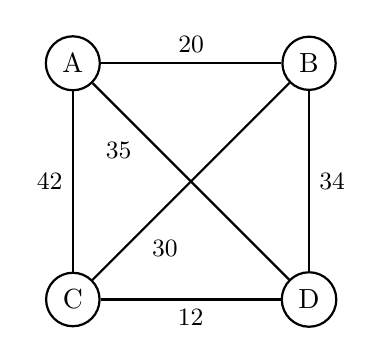
\begin{tikzpicture}[auto,node distance=3cm,
 thick,main node/.style={circle,draw}]
 \node[main node](A)[]{A};
 \node[main node](B)[right of = A]{B};
 \foreach \s/\t in {C/A, D/B}{ 
     \node[main node](\s)[below of = \t]{\s};}

\foreach \s/\t/\r in {A/B/20, C/A/42, B/D/34, D/C/12}{
    \path[draw, every node/.style={font=\small}] (\s) edge node{\r} (\t);}
 \foreach \s/\t/\r in {D/A/35, B/C/30}{
    \path[draw, every node/.style={font=\small},near end] (\s) edge node{\r} (\t);}  
 \end{tikzpicture}
\end{center}
\column{.5\textwidth}
Exhaustive Approach:
\begin{itemize}
\only<1>{
\item ABCDA = 97
\item ABDCA = 108
\item ACDBA = 108
\item ACBDA = 141
\item ADBCA = 141
\item ADCBA = 97
\item ...
}
\only<2>{
\item $n=4 \implies (n-1)!$ paths
\item reverse paths are the same so $\frac{(n-1)!}{2}$ paths to check

 }
\end{itemize}
\end{columns}
\end{frame}
%-----------------------------------------
\begin{frame}
\frametitle{Traveling Salesman Problem}

\begin{itemize}

\item Held-Karp Dynamic programming $O(2^n n^2)$
\item Heuristics - approxiamation to simplify, not necessarily correct
\item can get polynomial time
\item 2 types
 \begin{itemize}
 \item Build a path: Nearest Neighbor, Christofides
 \item Improve a path: K-opt, Lin-Kernighan
 \end{itemize}
\end{itemize}

\end{frame}
%----------------------------------------
\begin{frame}
\frametitle{TSP Heuristics}

\begin{itemize}
\item Simplest: Nearest Neighbor (Greedy) algorithm
 \begin{itemize}
 \item Pick a starting node
 \item Travel to the nearest neighbor
 \end{itemize}
\item Different answers depending on starting node
\item On average 25\% longer than optimal
\item $O(\log|n|)$
\end{itemize}


\end{frame}
%-------------------------------------------
\begin{frame}
\frametitle{TSP - Nearest Neighbor}
Start at 1.
\begin{columns}[c]

\column{.5\textwidth}
\begin{center}

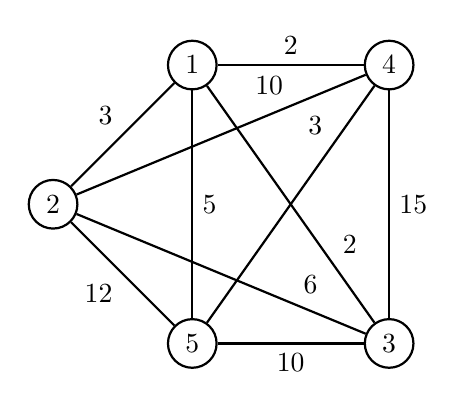
\begin{tikzpicture}[auto,node distance=2.5cm,
 thick,main node/.style={circle,draw}]
 
  \node[main node] (1) [] {1};
  \node[main node] (2) [below left of=1] {2};
  \node[main node] (4)  [right of=1] {4};
  \node[main node] (5) [below right of=2] {5};  
  \node[main node] (3) [ right of=5] {3};
  
  
  \foreach \s/\t/\i in {2/1/3, 1/4/2, 5/2/12, 4/3/15, 3/5/10,1/5/5 } {
   \path[draw] (\s) edge node {\i} (\t);}
  \foreach \s/\t/\i in {1/3/2,  2/3/6, 2/4/10, 5/4/3 } {
   \path[draw, near end] (\s) edge node {\i} (\t);}
\end{tikzpicture}
\end{center}

\column{.5\textwidth}
\begin{center}

\begin{tikzpicture}[auto,node distance=2.5cm,
 thick,main node/.style={circle,draw}]
 
  \node[main node] (1) [] {1};
  \node[main node] (2) [below left of=1] {2};
  \node[main node] (4)  [right of=1] {4};
  \node[main node] (5) [below right of=2] {5};  
  \node[main node] (3) [ right of=5] {3};
  
  \only<2->{\path[draw] (1) edge node {2} (4);}
  \only<3->{\path[draw, near end] (5) edge node {3} (4);}
  \only<4->{\path[draw] (3) edge node {10} (5);}
  \only<5->{\path[draw, near end] (2) edge node {6} (3);}
  \only<6->{\path[draw] (1) edge node {3} (2);}
\end{tikzpicture}
\end{center}
\end{columns}
\only<6->{Total weight: 24}
\end{frame}
%-------------------------------------------
\begin{frame}
\frametitle{TSP - NN}
Start at 5.
\begin{columns}[c]

\column{.5\textwidth}
\begin{center}

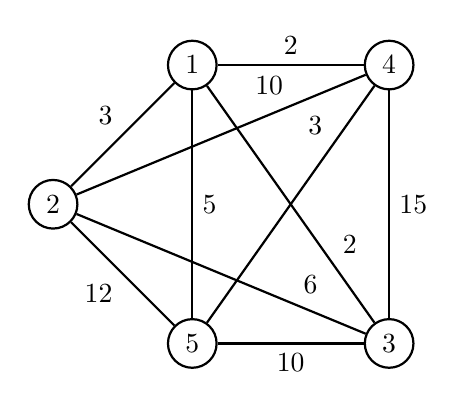
\begin{tikzpicture}[auto,node distance=2.5cm,
 thick,main node/.style={circle,draw}]
 
  \node[main node] (1) [] {1};
  \node[main node] (2) [below left of=1] {2};
  \node[main node] (4)  [right of=1] {4};
  \node[main node] (5) [below right of=2] {5};  
  \node[main node] (3) [ right of=5] {3};
  
  
  \foreach \s/\t/\i in {2/1/3, 1/4/2, 5/2/12, 4/3/15, 3/5/10,1/5/5 } {
   \path[draw] (\s) edge node {\i} (\t);}
  \foreach \s/\t/\i in {1/3/2,  2/3/6, 2/4/10, 5/4/3 } {
   \path[draw, near end] (\s) edge node {\i} (\t);}
\end{tikzpicture}
\end{center}

\column{.5\textwidth}
\begin{center}

\begin{tikzpicture}[auto,node distance=2.5cm,
 thick,main node/.style={circle,draw}]
 
  \node[main node] (1) [] {1};
  \node[main node] (2) [below left of=1] {2};
  \node[main node] (4)  [right of=1] {4};
  \node[main node] (5) [below right of=2] {5};  
  \node[main node] (3) [ right of=5] {3};
  
  \only<2->{\path[draw] (1) edge node {5} (5);}
  \only<3->{\path[draw] (1) edge node {2} (4);}
  \only<4->{\path[draw, near end] (2) edge node {10} (4);}
  \only<5->{\path[draw, near end] (2) edge node {6} (3);}
  \only<6->{\path[draw] (3) edge node {10} (5);}
\end{tikzpicture}
\end{center}
\end{columns}
\only<6->{Total weight: 33}
\end{frame}
%-------------------------------------
\begin{frame}
\frametitle{TSP - Held-Karp}
\begin{itemize}
\only<1>{
\item cities $1, 2, 3, ... n$
\item start at city 1
\item distance between cities $i$ and $j$ is $d_{ij}$
}
\only<2>{
\item for $S \subseteq \{2, 3, ... n\}$ and city $c$, let $D(S,c)$ be the minimum distance of starting at city 1, visiting all cities in $S$, and finishing at $c$.
\item If $S = \{c\}$ then $D(S,c) = d_{1c}$
\item otherwise $D(S,c) = \text{min}_{x \in S-\{c\} }(D(S-\{c\},x) + d_{xc}$
\item Goal: $D(\{2,3,...n\},1)$
}
\end{itemize}

\end{frame}
%----------------------------------
\begin{frame}
\frametitle{TSP - Held-Karp Notation Example}

Adjacency Matrix d:
\[
\begin{tabular}{|cccc|}
0 & 2 & 9 & 10 \\
1 & 0 & 6 & 4 \\
15 & 7 & 0 & 8 \\
6 & 3 & 12 & 0
\end{tabular}
\]

\begin{itemize}
\only<1>{
\item $|S| = 1$
\item $D(\{2\},3) = d_{32} + D(\empty, 2) = d_{32} + d_{21} = 7+1 = 8$
\item $D(\{3\},2) = d_{23} + D(\empty, 3) = d_{23} + d_{31} = 6+15 = 21$

}
\only<2>{
\item $|S| = 2$
\item $D(\{2,3\},4) = \text{min}\{  d_{42} + D(\{3\},2), d_{43} + D(\{2\},3)\}$

$= \text{min}\{3+21, 12+8\} = \text{min} \{24, 20\} = 20 $
}
\end{itemize}



\end{frame}
%------------------------------------
\begin{frame}
\frametitle{Held-Karp Example}
%\[
%\begin{tabular}{cccccc}
%\multicolumn{6}{c}{$D(\{2,3,4\},1)$}\\
%\multicolumn{2}{c}{$=\text{min}\{d_{12} + D(\{3,4\},2)$,}& \multicolumn{2}{c}{$d_{13} + D(\{2,4\},3)$,}&\multicolumn{2}{c}{$d_{14} + D(\{2,3\},4)\}}$\\
%$\{d_{24} + D(\{3\},4)$, & $d_{23} + D(\{4\},3)\}$ & $\{d_{32} + D(\{4\},2)$, & $d_{34} + D(\{2\},4)\}$ & $\{d_{42} + D(\{3\},2)$, & $d_{43} + D(\{2\},3)\}$


%\end{tabular}
%\]

$$D(\{2,3,4\},1)=\text{min}\{d_{12} + D(\{3,4\},2), d_{13} + D(\{2,4\},3), d_{14} + D(\{2,3\},4)\}$$
\pause
$$D(\{3,4\},2) = \text{min}\{d_{24} + D(\{3\},4), d_{23} + D(\{4\},3)\}$$
$$ D(\{2,4\},3) = \text{min}\{d_{32} + D(\{4\},2),  d_{34} + D(\{2\},4)\}$$
$$ D(\{2,3\},4) =  \text{min}\{d_{42} + D(\{3\},2),    d_{43} + D(\{2\},3)\}$$

\pause
\begin{columns}[c]
\column{.5\textwidth}
$$D(\{3\},4) = d_{43} + d_{31} = 12+15 = 27$$
$$D(\{4\},2) = d_{24} + d_{41} = 4+6 = 10$$
$$D(\{3\},2) = d_{23} + d_{31} = 6+15 = 21$$
\column{.5\textwidth}
$$D(\{4\},3) = d_{34} + d_{41} = 8+6 = 14$$
$$D(\{2\},4) = d_{42} + d_{21} = 3+1 = 4$$
$$D(\{2\},3) = d_{32} + d_{21} = 7+1 = 8$$
\end{columns}

\end{frame}

%--------------------------------------
\begin{frame}
\frametitle{Held-Karp Example}

$$D(\{2,3,4\},1)=\text{min}\{d_{12} + D(\{3,4\},2), d_{13} + D(\{2,4\},3), d_{14} + D(\{2,3\},4)\}$$

$$D(\{3,4\},2) = \text{min}\{d_{24} + D(\{3\},4), d_{23} + D(\{4\},3)\} $$
$$= \text{min}\{4 + 27 , 6 + 14\} = 20$$
$$ D(\{2,4\},3) = \text{min}\{d_{32} + D(\{4\},2),  d_{34} + D(\{2\},4)\}$$
$$= \text{min}\{7 + 10, 8 + 4\}  = 12$$
$$ D(\{2,3\},4) =  \text{min}\{d_{42} + D(\{3\},2),    d_{43} + D(\{2\},3)\} $$
$$=\text{min}\{3 + 21, 12 + 8\}  = 20$$


\end{frame}
%--------------------------------------
\begin{frame}
\frametitle{Held-Karp Example}

$$D(\{2,3,4\},1)=\text{min}\{d_{12} + D(\{3,4\},2), d_{13} + D(\{2,4\},3), d_{14} + D(\{2,3\},4)\}$$
$$ = \text{min}\{2+ 20, 9+ 12, 10+ 20\} $$
$$ = 21$$

path = \{1,3,4,2,1\}


\end{frame}




\end{document}